\documentclass[12pt]{article}
\usepackage[english]{babel}
\usepackage[utf8x]{inputenc}
\usepackage[T1]{fontenc}
\usepackage{scribe}
\usepackage{listings}
\usepackage{fullpage}
\usepackage{amsfonts}
\usepackage{amssymb}
\usepackage{hyperref}
\usepackage{url}

\usepackage[svgnames]{xcolor}
\usepackage{color}
% \definecolor{light-gray}{gray}{0.90}
% \lstset{backgroundcolor=\color{light-gray},showlines=true}

% \usepackage{xcolor}
% \usepackage{listings}

% \lstdefinestyle{BashInputStyle}{
%   language=bash,
%   basicstyle=\small\sffamily,
%   numbers=left,
%   numberstyle=\tiny,
%   numbersep=3pt,
%   frame=tb,
%   columns=fullflexible,
%   backgroundcolor=\color{yellow!20},
%   linewidth=0.9\linewidth,
%   xleftmargin=0.1\linewidth
% }


\usepackage{minted}
\setminted{fontsize=\footnotesize,baselinestretch=0.5}



\Scribe{}
\Lecturer{Queenie Qiu, John Raiti. Student: \textbf{Shucheng Guo, Harry Tung, Joshua Sanchez}}
\LectureNumber{3}
\LectureDate{DATE: Jan 26th. 2023}
\LectureTitle{Physical Implementations and Introduction to Control}

\lstset{style=mystyle}

\begin{document}
	\MakeScribeTop

%#############################################################
%#############################################################
%#############################################################
%#############################################################


\section {Sensor inaccuracies in the physical robot}
\subsection{Connecting to the physical robot}
Connecting to the physical robot according to the instructions in the slides. 


\subsection{Errors in odometry in real world operation}

In this section, we will use the patrol example that we have explored in the Lab1 again so as to compare the odometry performance between simulation and real world implementation. We will use the nodes and code created in Lab1 to visualize data from the /odom topic.    

\textbf{Deliverables:}
\begin{enumerate}
    
    \item Run the patrol example with the following parameters: square length 0.8m and 1 iteration. In an additional terminal run the plot\_odom.py file.
    
    \begin{minted}{bash}
      $ roslaunch turtlebot3_example turtlebot3_client.launch
      
      $ rosrun turtlebot3_example turtlebot3_server
    \end{minted}

    \begin{enumerate}

        \item Make notes about robot behaviors: do the wheels turn at the same rate when moving forward? Were the 90 degree turns accurate? Does the robot return to the starting position?
        
        \textbf{Answer: }The wheels would rotate at the same rate when moving forward without the impact of other factors, e.g. low battery, facing obstacles.
        \\The turns, however, were far from accurate. The robot wouldn't make perpendicular turns in square patrols, not to mention gradual ones in circular turns. 

        \item Plot the x-y position of the robot against the “ground truth” and take a screenshot.
        
        \begin{figure}[H]
          \centering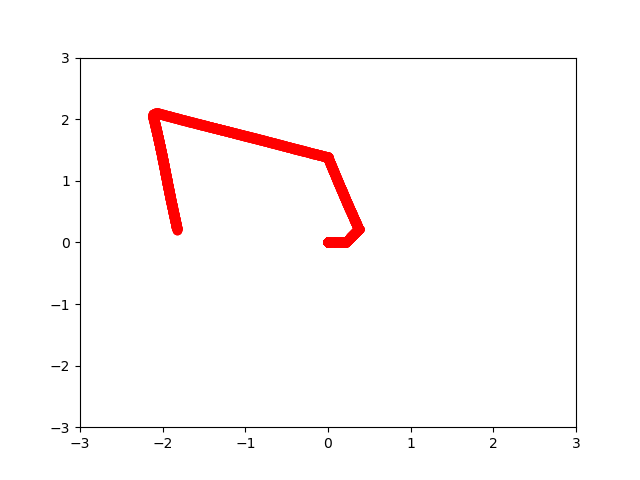
\includegraphics[width=14cm]{images/gmapping.png}\vspace{-10pt}
          \caption{Plotting robot patrol of \mintinline{bash}{s 0.8 1} on a 2D graph.}\label{fig:gmapping}
          \end{figure}

        \item Compare the graph to the one obtained in Lab1. Mention differences. Are odom errors larger or smaller? Mention what can be influencing the results.
    
    \end{enumerate}

    \item What can be done to improve the accuracy of sensor data or to get better estimation of robots' positions and orientations?
    


\end{enumerate}


\subsection{Errors in laser readings in real world operation}
In this section, we will go through the mapping procedure followed in Lab2, and store the /scan topic data into a rosbag. We will compare the gmapping results in the real world against the ones obtained in the simulation.

\begin{enumerate}
    \item Make sure the physical turtlebot is operational and placed correctly, in the environment you want to map. Move the robot to the right bottom corner of the map. 
    \begin{figure}[H]
    \vspace{-10pt}
    \centering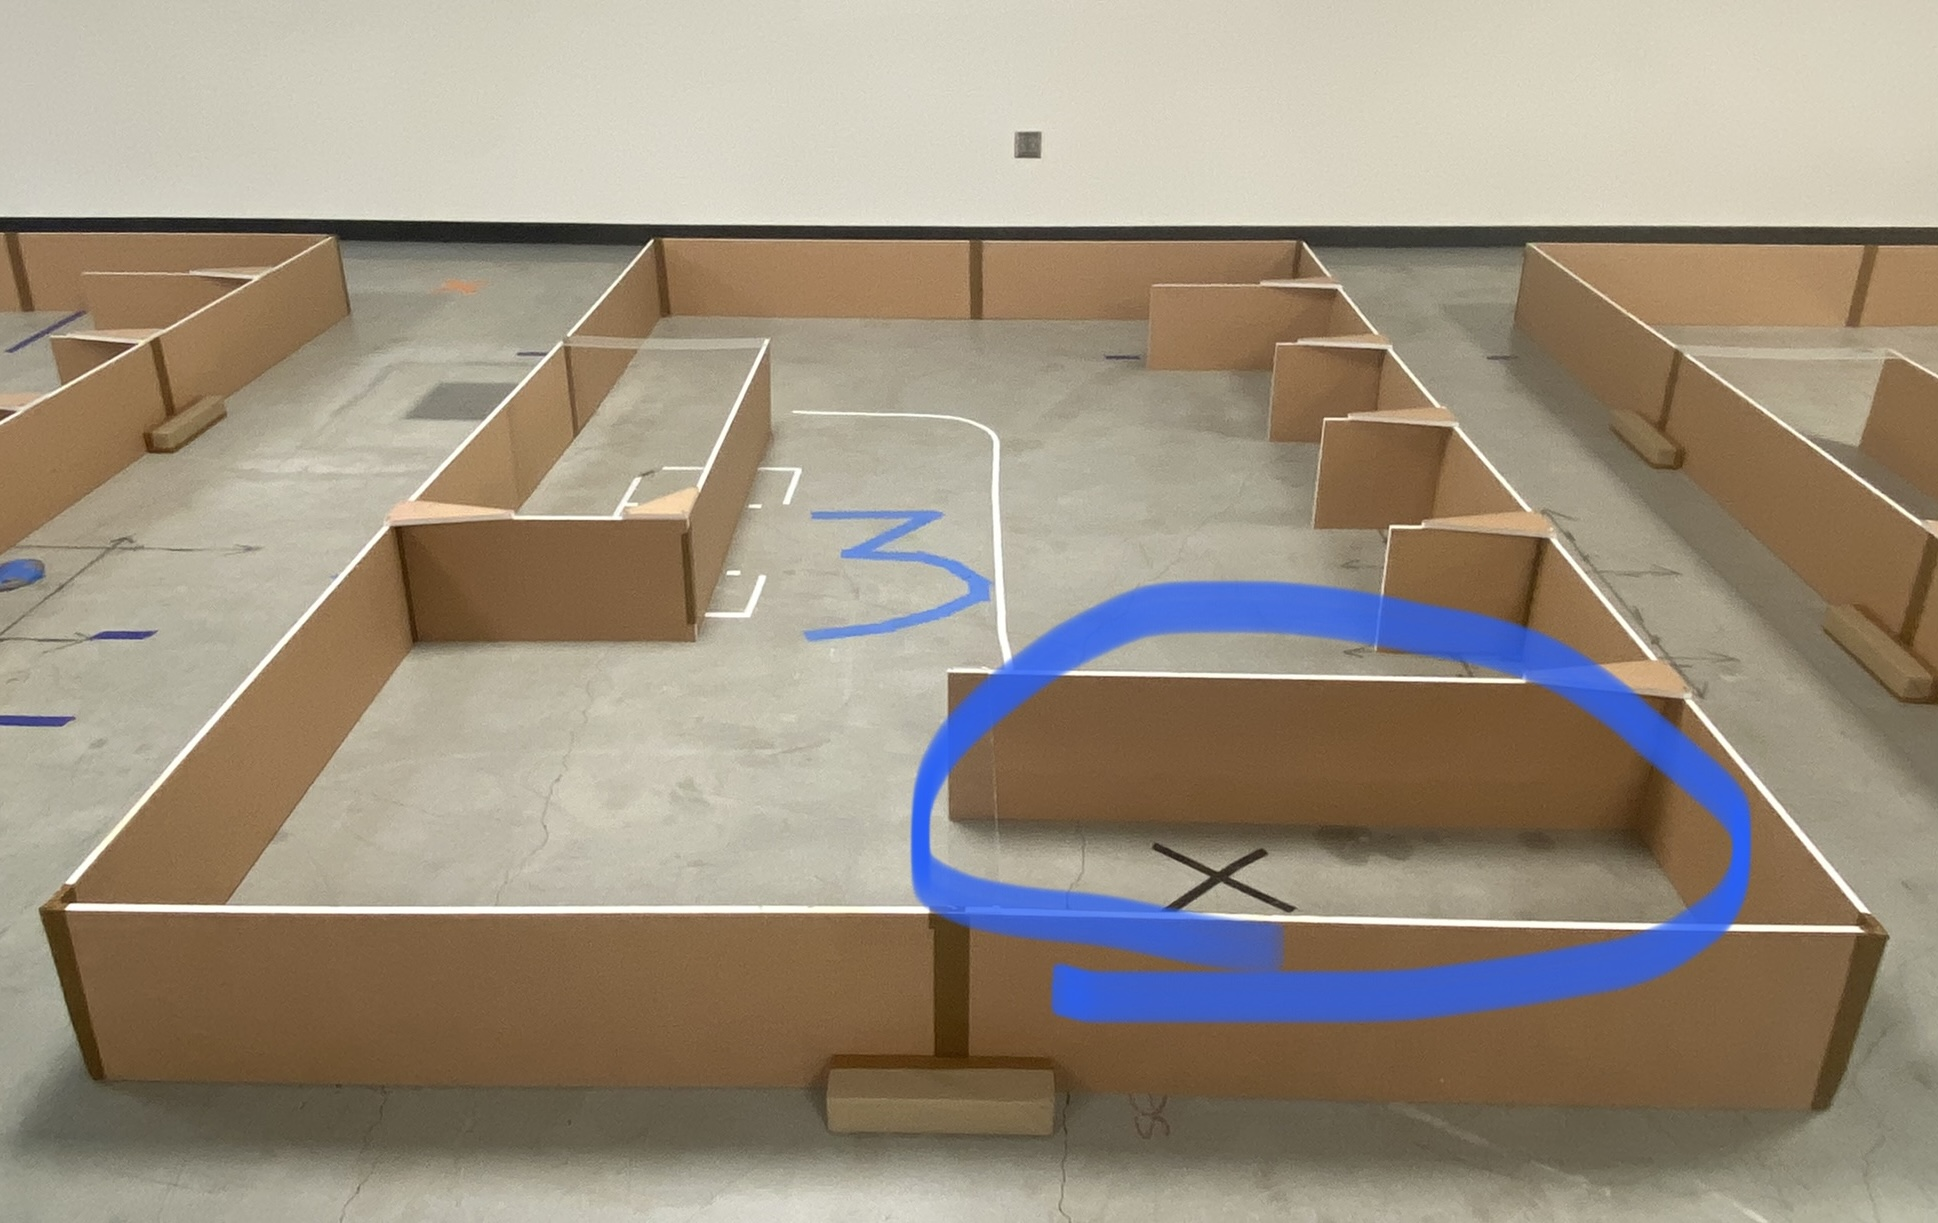
\includegraphics[width=14cm]{images/map.jpeg}\vspace{-10pt}
    \caption{Start Position Indication}\label{fig:pid}
    \end{figure}
    
    As a reminder the command line to launch the mapping is as follows:
    \begin{minted}{bash}
    $ roslaunch turtlebot3_slam turtlebot3_slam.launch slam_methods:=gmapping
    \end{minted}
    Note: you will need to run the teleoperation program to go through the map.
    \begin{minted}{bash}
    $ roslaunch turtlebot3_teleop turtlebot3_teleop_key.launch
    \end{minted}
    \item Additionally, before you start teleoperating the robot, record a rosbag file with the following topics.
    \begin{minted}{bash}
    $ rosbag record /odom /scan /cmd_vel /tf -O physicaltb3_map.bag
    \end{minted}
    
    \item When you have finished tracing the surroundings to complete the map, you can stop the bag file recording and save the resulting map by running the following command in the terminal before finishing the gmapping launch.
    \begin{minted}{bash}
        $ rosrun map_server map_saver -f ~/gix_map
    \end{minted}
    
    
\end{enumerate}

\textbf{Deliverables:}
\begin{enumerate}
    \item Inspect the resulting files of the maps: the one obtained in the simulation and the one from the physical implementation. Attach screenshots of both pgm files. Mention differences between the results obtained in the simulation and the real world in terms of: thickness of the edges, additional shapes outside of the intended map area, differences in parameter values found in the .yaml file.
    
    \item Use that map you just created and launch the navigation example in Lab2. Return the robot to the start position on the physical map. You may want to use that spot to give a 2DPoseEstimate as your starting position.
    \begin{minted}{bash}
        $ roslaunch turtlebot3_navigation turtlebot3_navigation.launch map_file
        :=$HOME/gix_map.yaml
    \end{minted}
    \begin{enumerate}
        \item Set a 2DNavGoal on the map that is close to this area.
        \begin{figure}[H]
        \vspace{-10pt}
        \centering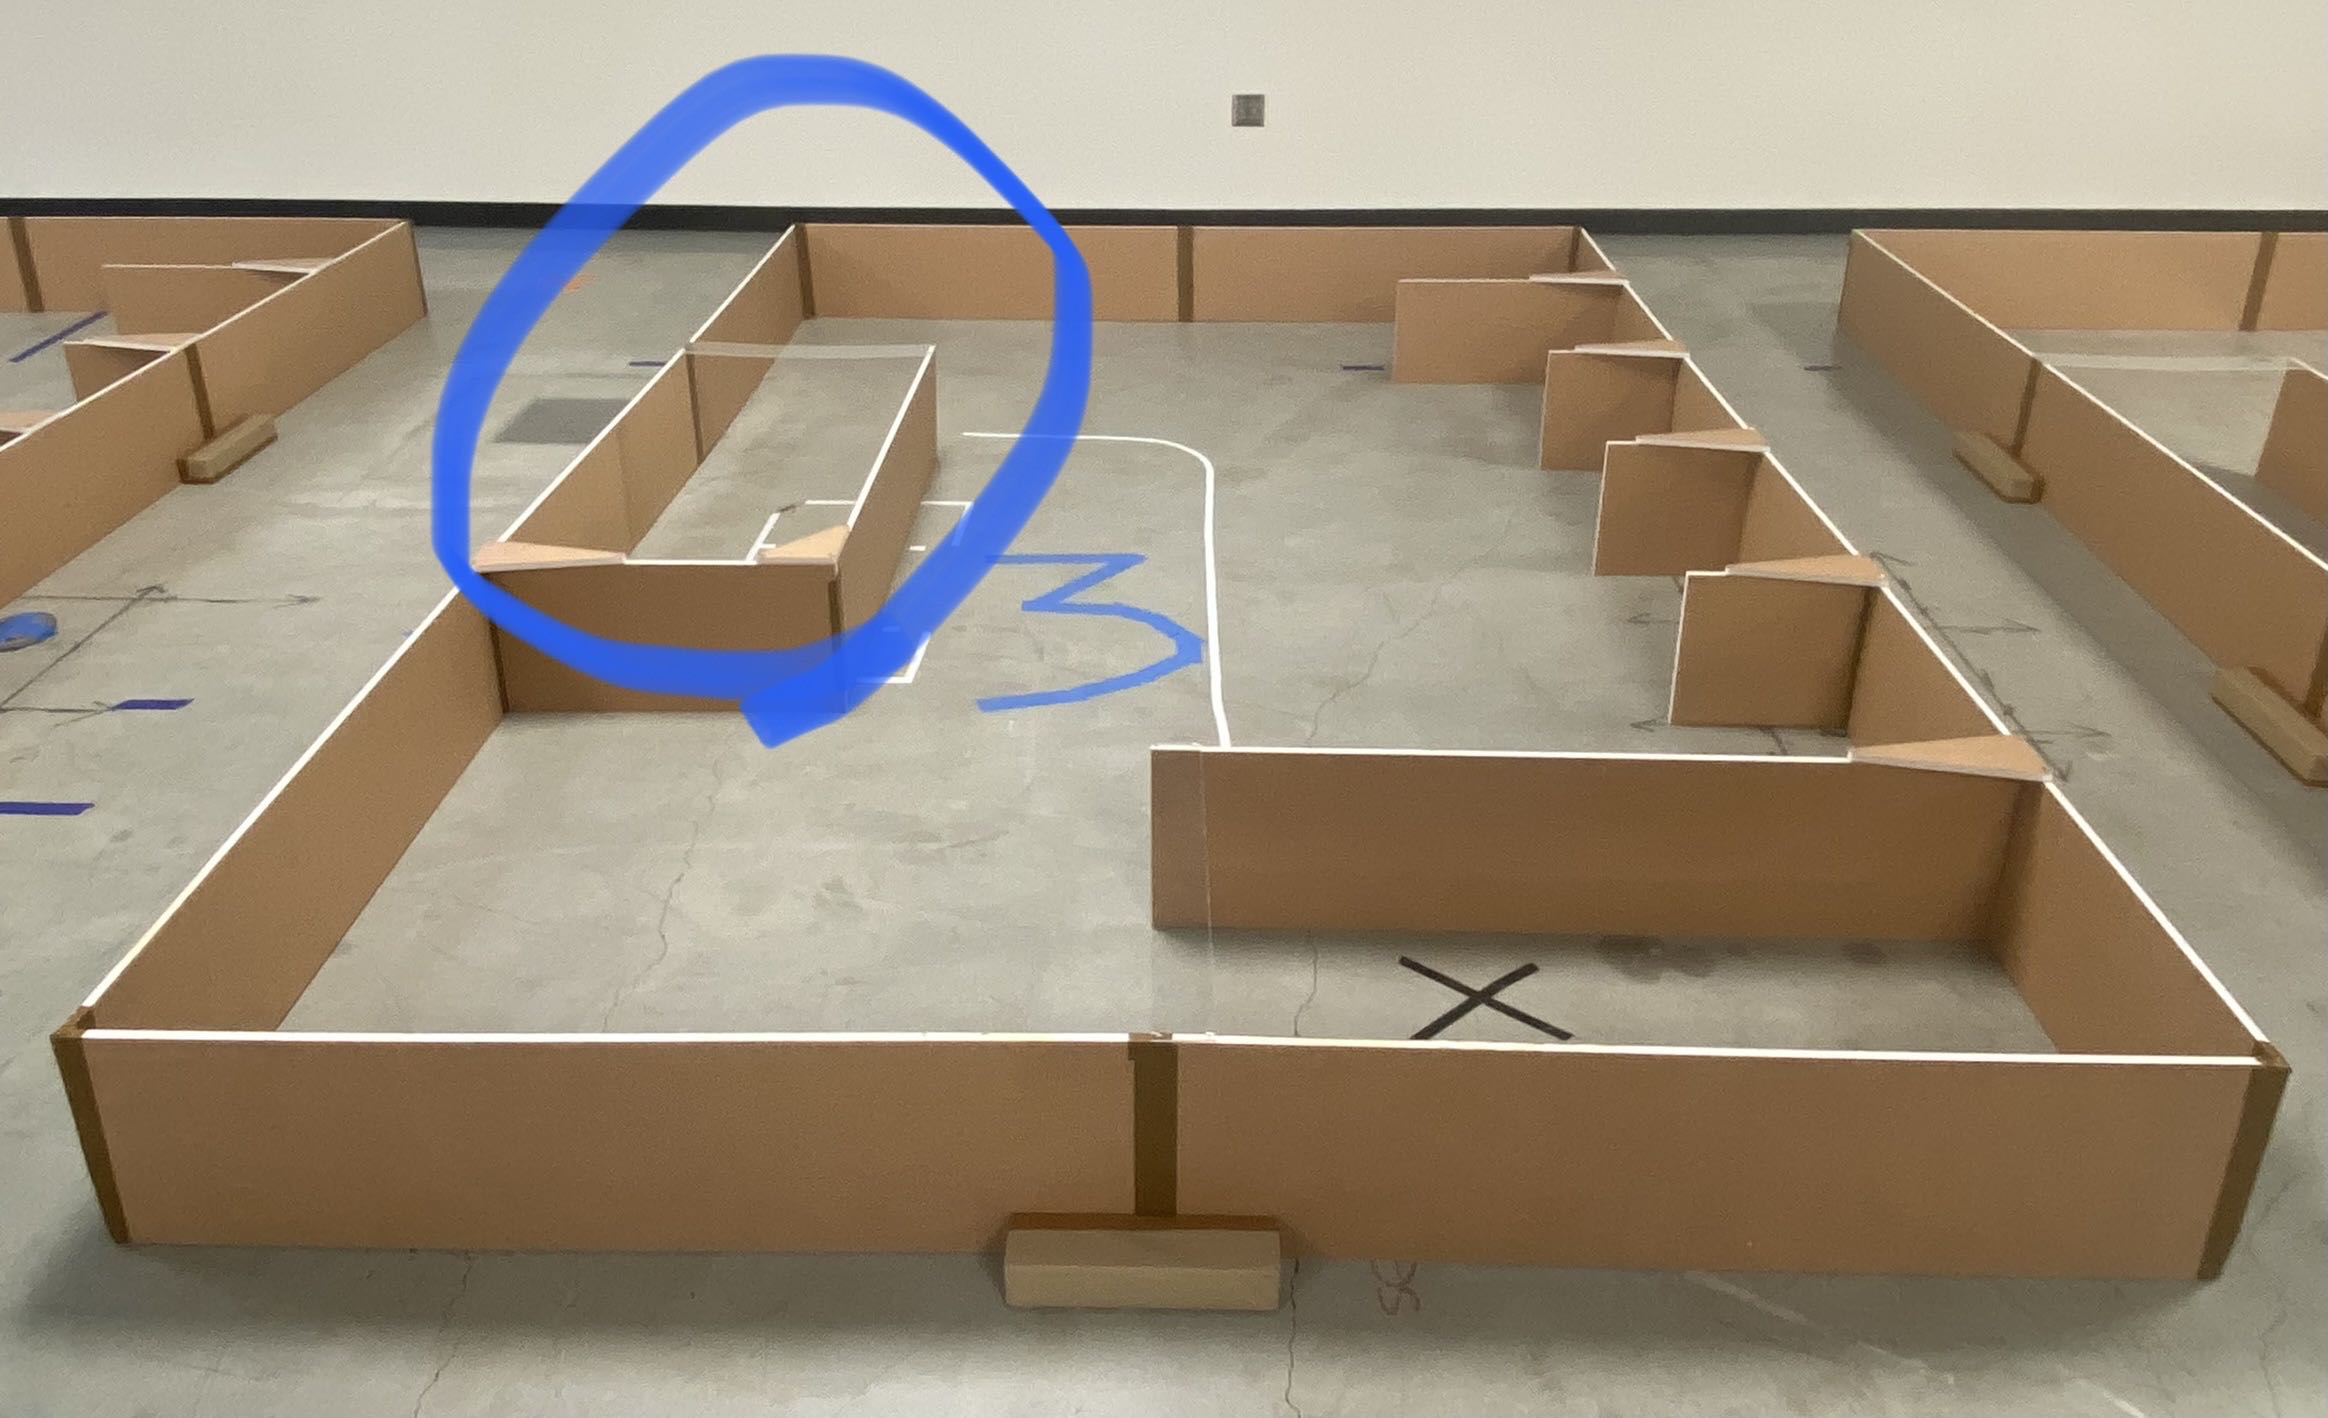
\includegraphics[width=14cm]{images/map2.jpeg}\vspace{-10pt}
        \caption{2DNavGoal Position Indication}
        \end{figure}
        
        What happens when a 2D navigation goal is provided? How long (time) does it take for your robot to plan and reach the goal? 
        \item How close did the robot get to the goal (distance from the goal)?
        \item Discuss your observations. These should include quantitative and qualitative components. You may rely on comparisons based on the concentric rings shown around the goal, or you may reference your comparisons to the robot’s interpretation of the world.
    \end{enumerate}
    \item Submit your recorded rosbag with your lab assignment.
    
    
\end{enumerate}

\textbf{The above section of the lab needs to be finished by the end of lab session on Jan 26th.} 


\section{Introduction to control strategies in robot navigation
}
In this section, we will explore different paradigms to control the movements of a robotic platform. In this case, we will focus on the changes in position and orientation of a wheeled robot. For convenience, we will return to the simulation setting.
This means that we will set our environment variables to its previous values of localhost in the .bashrc file. 

\subsection{Executing robot motions in open-loop control}

Open-loop refers to the robot’s operation created by the input signal does not depend on the system’s output. Specifically, we will create commands for the robot to move forward 1.5 meters.
\begin{enumerate}
    \item Launch a simulated turtlebot3 in the stage\_1 world.
    \begin{minted}{bash}
        $ roslaunch turtlebot3_gazebo turtlebot3_stage_1.launch
    \end{minted}
    \item By knowing the distance to be traveled, we can determine the constant speed and the amount of time that constant speed needs to be held to cover said distance. Use the command-tool rostopic to publish velocity commands to the robot:
    \begin{minted}{bash}
        $ rostopic pub -1 /cmd_vel geometry_msgs/
        Twist  '{linear:  {x: <value>, y: 0.0, z: 0.0}, angular
        : {x: 0.0,y: 0.0,z: 0.0}}'
    \end{minted}
    After a certain amount of time (pos = vel * time), you will publish a twist message to effectively stop the robot from moving:

    \begin{minted}{bash}
        $ rostopic pub -1 /cmd_vel geometry_msgs/Twist '{linear
        :  {x: 0, y: 0.0, z: 0.0}, angular: {x: 0.0,y: 0.0,z: 0.0}}'
    \end{minted}
    
    For your convenience, we have prepared a simple python script that submits the commands to the terminal by using the os library. You will need to complete your selected values for time and speed.
    
    
    
\end{enumerate}

\textbf{Deliverables:}
\begin{enumerate}
    \item Report the chosen strategy (published values) to complete the task of moving 1.5m forward in open-loop.
    
    \item Inspect the turtlebot3’s position in Gazebo. (World -> Models -> turtlebot3\_burger -> pose -> x). Did the robot move 1.5m accurately?
    
    \item Compare your desired traveled value of 1.5m with the actual position of the robot in gazebo, and the reported value in the /odom topic (use rostopic echo /odom). Discuss differences.
  
    \item Mention the challenges of operating the robot in open-loop, particularly when the motions increase in complexity.
    \item How would the sequence of commands look if you wanted to complete a patrol pattern (e.g. a triangle) in open-loop? Report the solution in pseudocode, commands should include GoForward(distance),WaitTime(time), Rotate(angle in degrees).
    \item Modify the given open loop file to achieve this patrol motion.
    \item How close to the start location did your robot finish? Use values from both: odometry and gazebo pose.
\end{enumerate}

\subsection{Executing robot motions in closed-loop control}
In closed-loop operation, the robot’s input signal depends on a reference value that we want the output to be, and the comparison against the robot’s current output through sensor feedback. We will create commands for the robot to move forward 1.5 meters by using the readings of some of its sensors, namely odometry and laser.

\begin{enumerate}
    \item Create a node that subscribes to the /odom topic and publishes to the /cmd\_vel topic. It will read the initial /odom value and only stop publishing commands to the velocity topic when the current value increases by 1.5m. Use the file close\_loop\_odom.py as a starting point.
    
    \item Create a node that subscribes to the /scan topic and publishes to the /cmd\_vel topic. It will read the initial /scan value corresponding to the front of the robot and only stop publishing commands to the velocity topic when the current scan value decreases by 1.5m. Use the file close\_loop\_laser.py as a starting point.

\end{enumerate}

\textbf{Deliverables:}
Run your closed-loop nodes to move the robot 1.5 meters forward and compare the performance of using /odom vs. /scan. Also check the robot’s position in Gazebo through the plotting utility and compare to answer following questions:
\begin{enumerate}
    \item How do each closed-loop control compare to the open-loop performance?
    \item Record a video of the robot’s performance for each closed-loop control node. Attach your video links.
\end{enumerate}

\section{Extra credit: Simulated Wall-following behavior}
Now that we have completed motion using open and closed-loop control, we will go further into closed-loop by adding a controller step. Instead of using the error between the difference of an output measurement of our system and a specified reference value, the controller will use this error as input and output values to be used directly by the system. In our particular case of the simulated turtlebot3, we will use the readings from the laser sensor and a reference value of 0.5m to keep the robot driving parallel to a wall in the environment. 
We will provide code that you will need to complete, where a controller will use the error in the distance to the wall to output values from a PID controller that will modify the /cmd\_vel values

\begin{enumerate}
    \item Download the wall\_follower and PID python files from the course materials and add them to your workspace (e.g. turtlebot3/turtlebot3\_example/nodes folder). You will need to use the chmod +x <filename> command to make both files executables.
    \begin{minted}{bash}
        $ rosrun turtlebot3_example wall_follower.py
    \end{minted}
    
    \item Complete the code by selecting the correct topics to subscribe and publish, making sure that the readings from the lidar sensor are used correctly (you are interested in keeping a wall to the right side of the robot at a 0.5 distance at all times, this maps to a specific position in the ranges array).
    
    \item Launch a simulated turtlebot3 burger in the empty world in Gazebo. Change the initial position of the turtlebot3.
    \begin{minted}{bash}
        $ roslaunch turtlebot3_gazebo turtlebot3_empty_world.launch x_pos
        :=-19.0 y_pos:=0.0
    \end{minted}
    
    \item Go to the Insert model tab in Gazebo’s left panel and add a “Grey Wall”. Go into the Model Editor to modify the geometry of the link in both visual and collisions tab (X = 20.0). Set the pose of the new long grey wall to x=-0.8, y=0.0
    
    \item Run (rosrun) the wall\_follower node. We will change the values in the main function of the file to modify the PID controller parameters and observe performance. Every time you terminate the launch you need to publish a /cmd\_vel message with zeros to stop the turtlebot3. You also need to reset the world poses in Gazebo (Ctrl+Shift+R). This step may have to be done several times before you see the robot in its original pose.
    
    
\end{enumerate}

\textbf{Deliverables}
\begin{enumerate}
    \item Run the plotting node (plot\_odom.py) to visualize the change of the error value over time with the different PID parameters values and save the plots for each case. You can also use the Gazebo plotting Utility and export the resulting plot.
    
    \item Describe what is happening in each of the 6 plots you create. For example: time for error to go to zero, is it oscillating, is there stationary error?
    
    \begin{figure}[H]
    \vspace{-10pt}
    \centering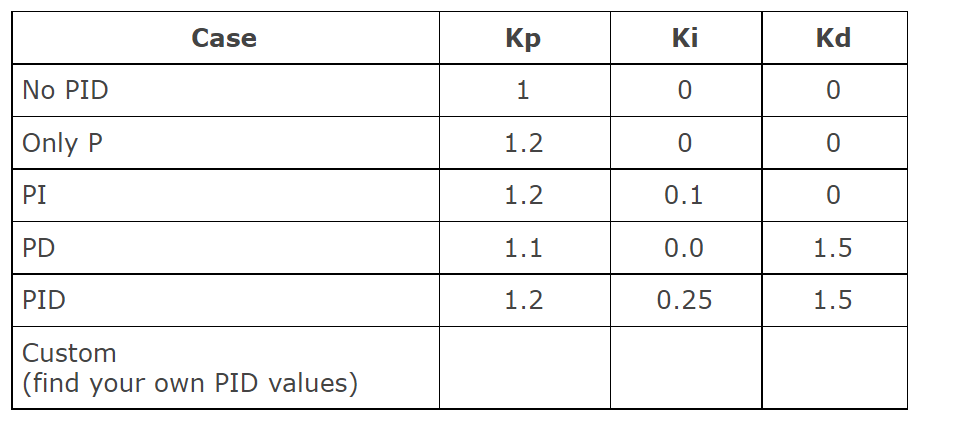
\includegraphics[width=14cm]{images/pidparameter.png}\vspace{-10pt}
    \caption{Parameters for PID.}\label{fig:pid}
    \end{figure}
    
    For the custom values of the PID, you should aim to have a response that goes fast to the desired reference, has little or no oscillation in the response and its response is centered on the desired response (no stationary error)
    
    \item Compare the performance of the six controllers mentioned in the previous table in terms of:
    a. Time it takes to reach the desired goal (error=0).
    b. Peak oscillation value.
    c. Stationary error (value at which the robot settles and moves forward).
    
    \item Describe some of the challenges you faced with this wall following task and the steps you took to overcome them.
    
    \item Mention at least 2 applications where PID controllers would be useful to a robotic implementation (e.g. navigation)
\end{enumerate}


\end{document}